\textbf{NOTE: We have already demoed to the TA for this course and have proven that our implementation of the HTTP web server is correct and in working order.}
     \begin{figure}[!htbp]
        \frame{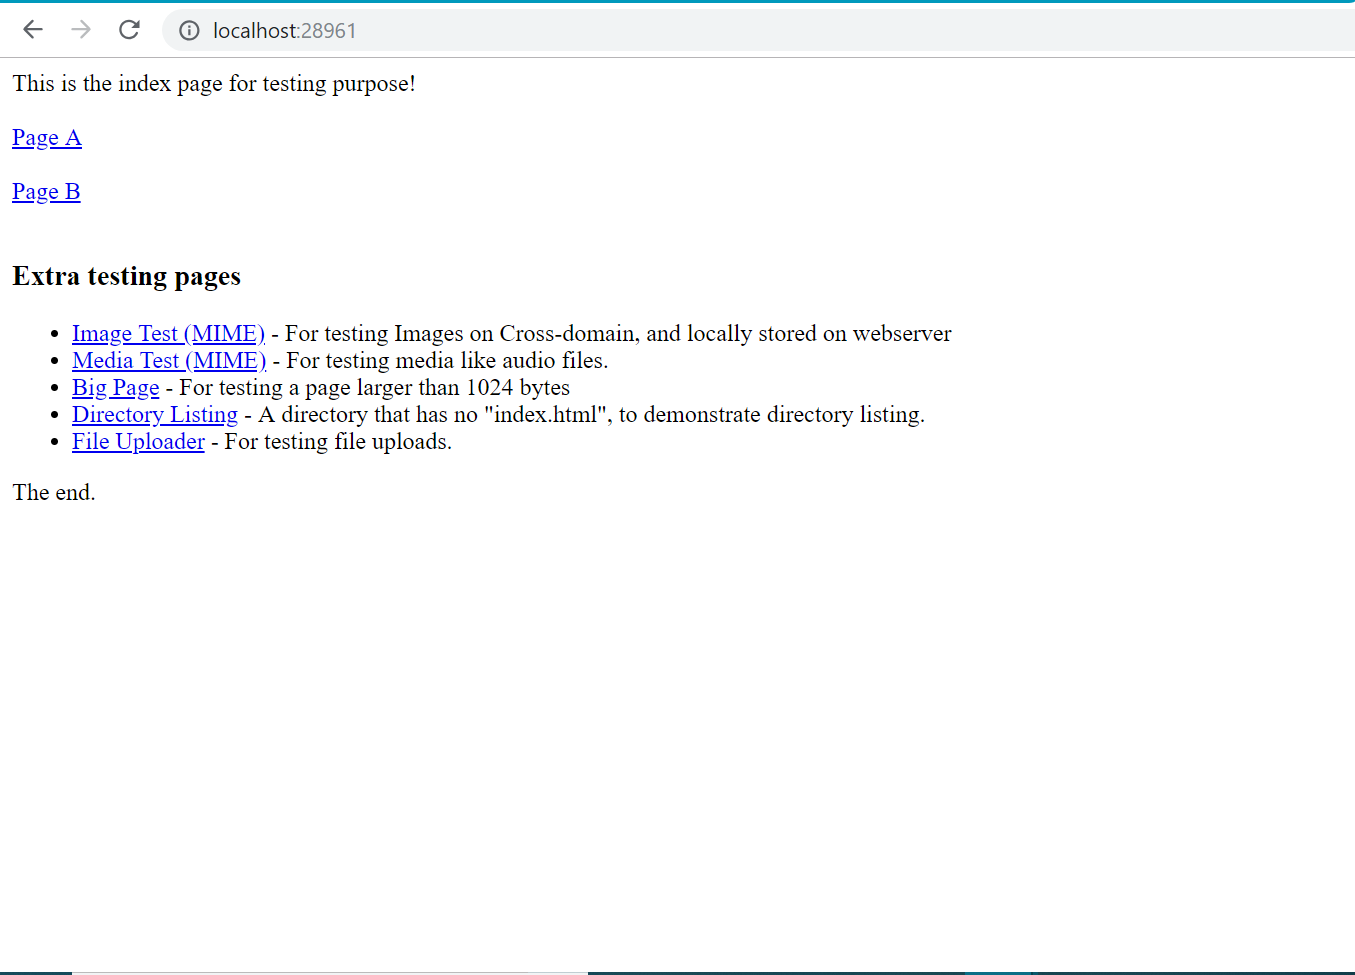
\includegraphics[width=\textwidth]{indexpage.PNG}}
        \caption{The figure above shows the index.html page of the webserver.}
    \end{figure}
         \begin{figure}[!htbp]
  \frame{
\includegraphics[width=\textwidth]{pageA.PNG}}
  \caption{The figure above shows the additional page, Page A, in the webserver.}
\end{figure}
     \begin{figure}[!htbp]
 \frame{ 
\includegraphics[width=\textwidth]{pageB.PNG}}
  \caption{The figure above shows the additional page, Page B, in the webserver.}
\end{figure}
     \begin{figure}[!htbp]
 \frame{ 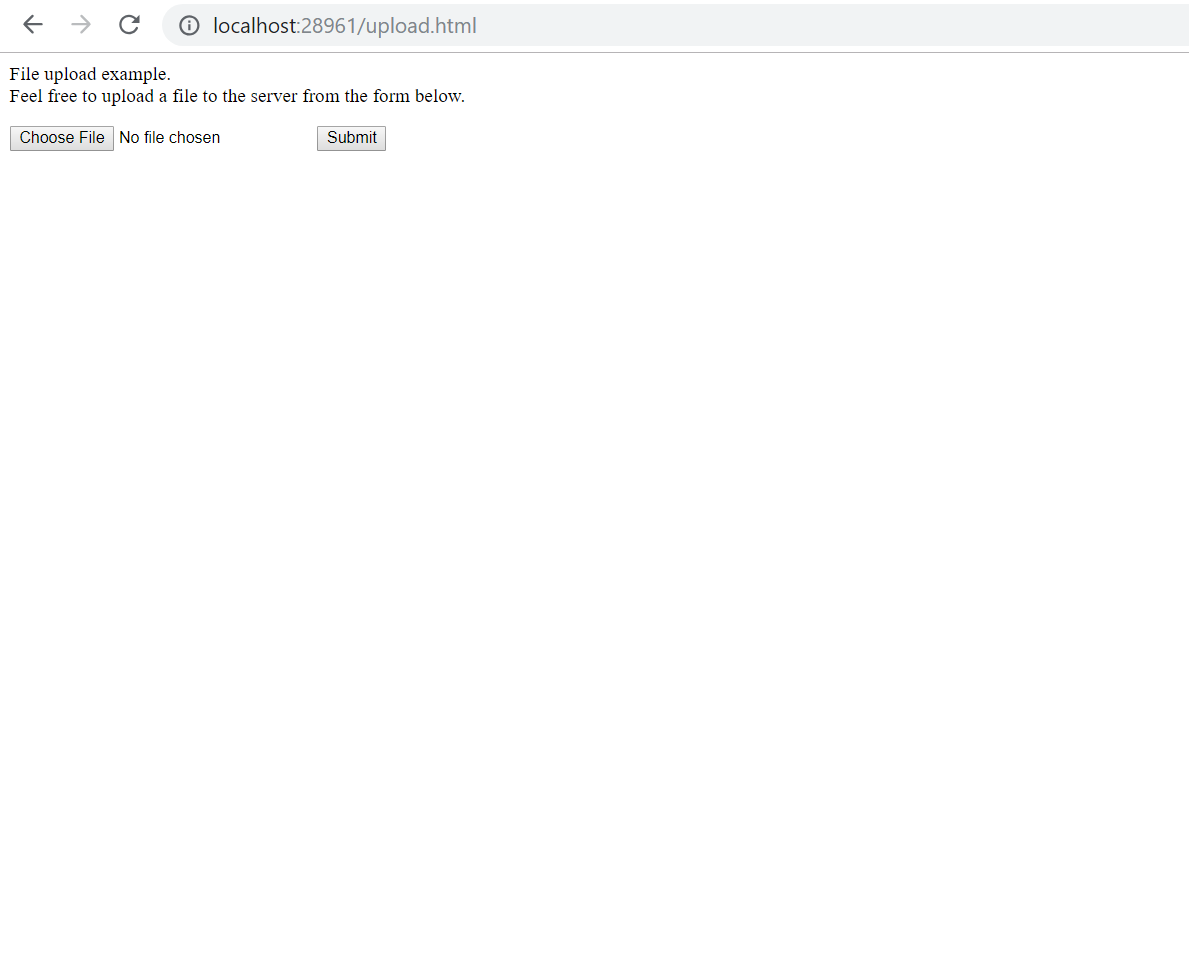
\includegraphics[width=\textwidth]{pageUpload.PNG}}
  \caption{The figure above shows the additional page, for uploading files.}
\end{figure}
     \begin{figure}[!htbp]
 \frame{ 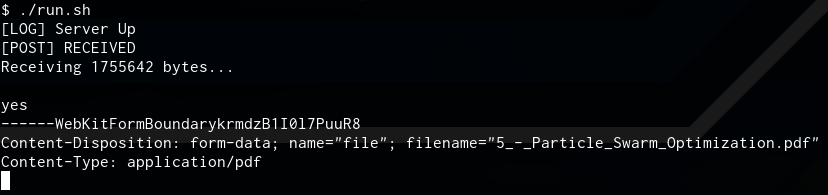
\includegraphics[width=\textwidth]{servergotfile.png}}
  \caption{The figure above that the server has received the request to upload the file.}
\end{figure}
     \begin{figure}[!htbp]
 \frame{ 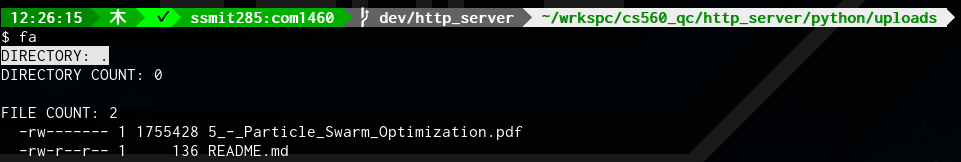
\includegraphics[width=\textwidth]{showserverhasfile.png}}
  \caption{The figure above shows that the server has uploaded the file and the file is now listed in the directory listing.}
\end{figure}
     \begin{figure}[!htbp]
 \frame{ 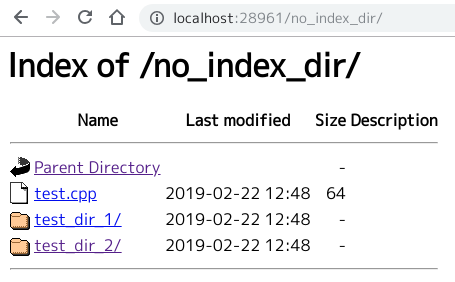
\includegraphics[width=\textwidth]{dirlist.png}}
  \caption{The figure above shows the directory listing page.}
\end{figure}
     \begin{figure}[!htbp]
 \frame{ 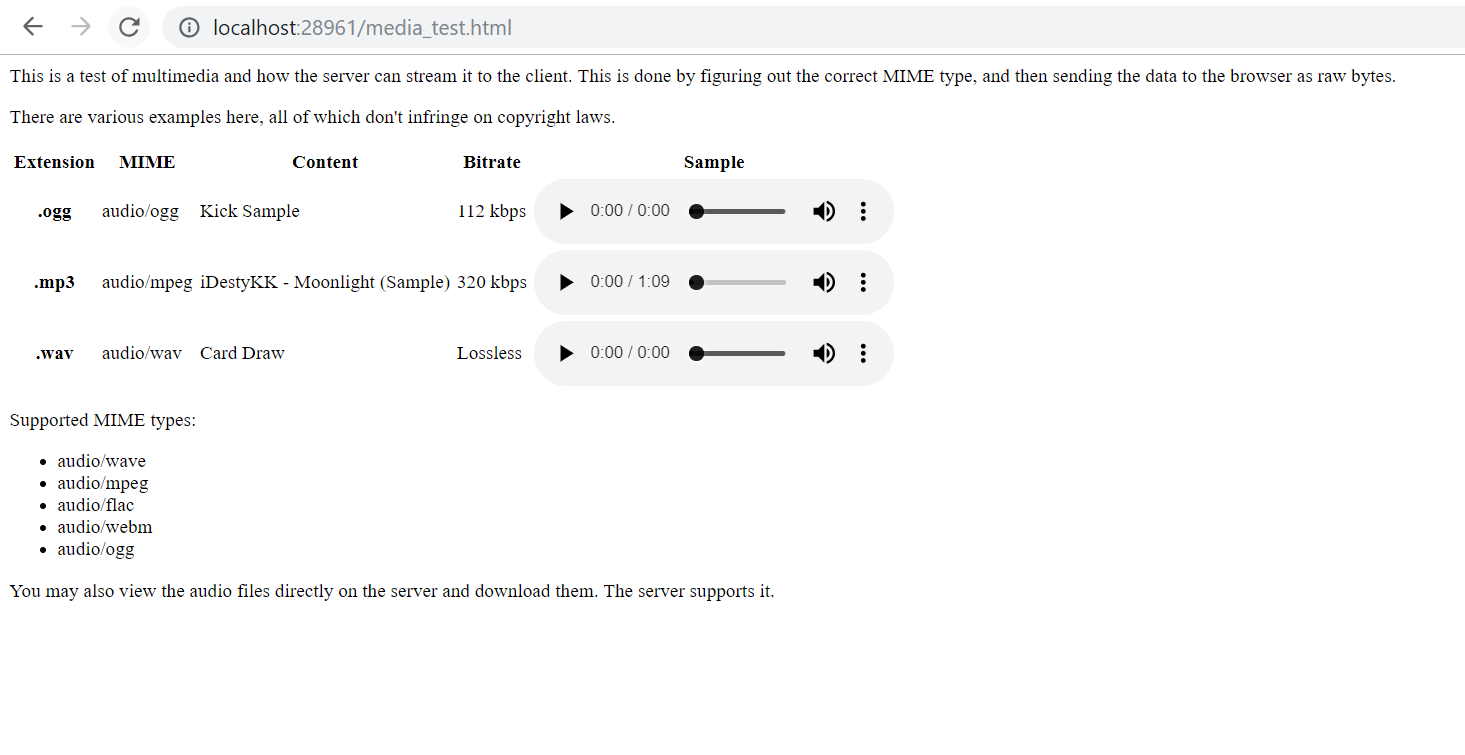
\includegraphics[width=\textwidth]{pageMedia.PNG}}
  \caption{The figure above shows the additional page, the Media Test Page, in the webserver. This was not a main requirement of the assignment, but was added in as an enhancement.}
\end{figure}
 \begin{figure}[!htbp]
 \frame{ 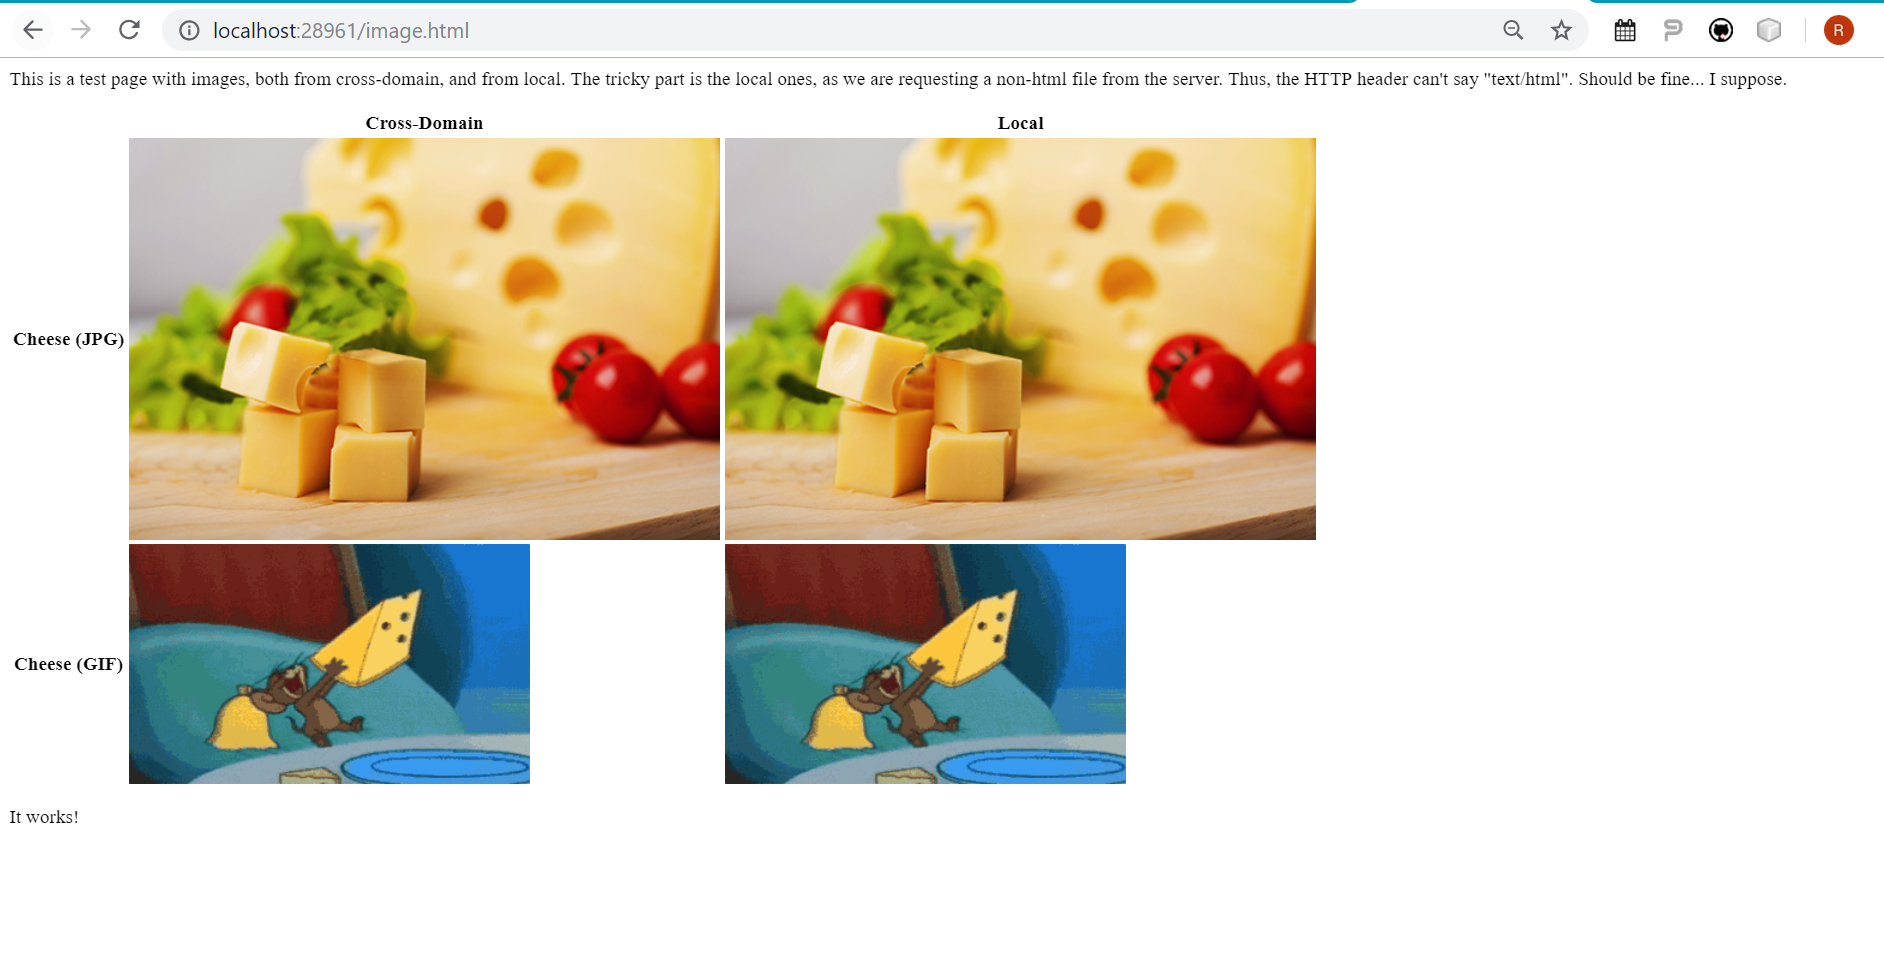
\includegraphics[width=\textwidth]{pageImage.PNG}}
  \caption{The figure above shows the additional page, the Image Test Page, in the webserver. This was not a main requirement of the assignment, but was added in as an enhancement. This page demonstrates locally hosted images and externally hosted images.}
\end{figure}
